% Build with pdflatex withdrawal_workflow_compact.tex.
\documentclass[border=.4mm]{standalone}
\usepackage[T1]{fontenc}
\usepackage{newtxtext}
\usepackage{tikz}
\usetikzlibrary{arrows.meta}
\definecolor{workflownavy}{HTML}{1C3F60}
\definecolor{workflowink}{HTML}{131820}
\definecolor{workflowheader}{HTML}{E2EDFA}
\definecolor{workflowline}{HTML}{B4C6D4}
\definecolor{workflowrr}{HTML}{777777}
\definecolor{workflowsa}{HTML}{D55E00}
\definecolor{workflowew}{HTML}{0072B2}

\newcommand{\workflowpanel}[3]{%
    \begin{scope}
        \clip[rounded corners=1.05mm] (#1,0) rectangle (#2,27.5);
        \fill[workflowheader] (#1,0) rectangle (#2,5);
        \draw[workflowline,line width=.4pt] (#1,5) -- (#2,5);
    \end{scope}
    \draw[workflownavy,line width=.55pt,rounded corners=1.05mm] (#1,0) rectangle (#2,27.5);
    \node[heading] at ({(#1+#2)/2},2.45) {#3};
}
\newcommand{\workflowarm}[3]{%
    \fill[#2!9,rounded corners=.6mm] (40.6,#1) rectangle (95.4,{#1+3.8});
    \node[anchor=west,inner sep=0pt,text=#2!72!black,font=\bfseries]
        at (42,{#1+1.9}) {#3};
}

\begin{document}
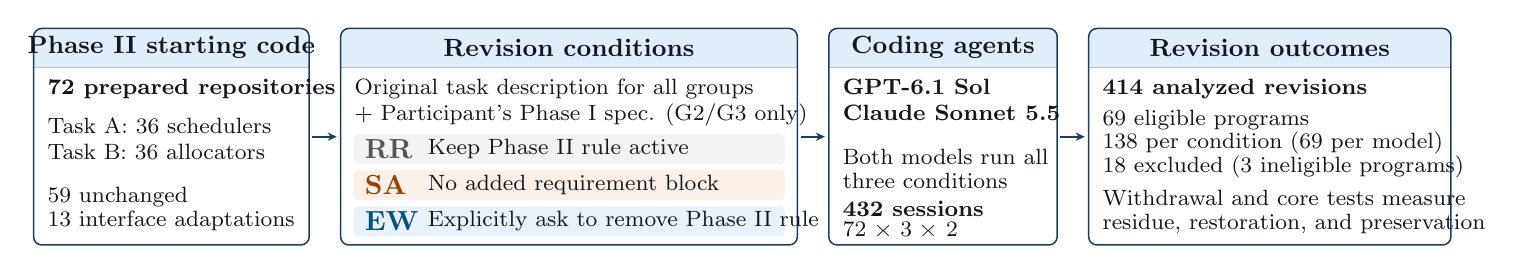
\begin{tikzpicture}[
    x=1mm,y=-1mm,text=workflowink,font=\fontsize{8.2}{9.3}\selectfont,
    heading/.style={inner sep=0pt,font=\fontsize{9.15}{10}\selectfont\bfseries},
    body/.style={anchor=north west,inner sep=0pt,align=left},
    small/.style={font=\fontsize{7.7}{8.6}\selectfont},
    flow/.style={draw=workflownavy,line width=.65pt,-{Stealth[length=1.15mm,width=1.05mm]}},
]
    \workflowpanel{0}{35}{Phase II starting code}
    \workflowpanel{39}{97}{Revision conditions}
    \workflowpanel{101}{130}{Coding agents}
    \workflowpanel{134}{180}{Revision outcomes}
    \foreach \x in {35,97,130}
        \draw[flow] ({\x+.4},13.75) -- ({\x+3.5},13.75);

    \node[body] at (1.7,6.4) {\textbf{72 prepared repositories}};
    \node[body] at (1.7,11.3) {Task A: 36 schedulers\\Task B: 36 allocators};
    \node[body,small] at (1.7,20.1) {59 unchanged\\13 interface adaptations};

    \node[body] at (40.7,6.4) {Original task description for all groups\\
        + Participant's Phase I spec. (G2/G3 only)};
    \workflowarm{13.4}{workflowrr}{RR}
    \workflowarm{18.0}{workflowsa}{SA}
    \workflowarm{22.6}{workflowew}{EW}
    \foreach \y/\label in {
        15.3/{Keep Phase II rule active},
        19.9/{No added requirement block},
        24.5/{Explicitly ask to remove Phase II rule}}
        \node[anchor=west,inner sep=0pt] at (50,\y) {\label};

    \node[body] at (102.7,6.4) {\textbf{GPT-6.1 Sol}\\\textbf{Claude Sonnet 5.5}};
    \node[body,small] at (102.7,15.3) {Both models run all\\three conditions};
    \node[body] at (102.7,21.8) {\textbf{432 sessions}};
    \node[body,small] at (102.7,24.5) {72 \texttimes\ 3 \texttimes\ 2};

    \node[body] at (135.7,6.4) {\textbf{414 analyzed revisions}};
    \node[body,small] at (135.7,10.25) {69 eligible programs\\
        138 per condition (69 per model)\\
        18 excluded (3 ineligible programs)};
    \node[body,small] at (135.7,20.45) {Withdrawal and core tests measure\\
        residue, restoration, and preservation};
\end{tikzpicture}
\end{document}
